\section{Accounting for latent organisation of the network}

\begin{frame}
  \frametitle{Handling with the data structure and scarcity}
  \framesubtitle{By introducing some prior}

  \begin{block}{Priors should be biologically grounded}
    \begin{enumerate}
    \item no too many genes effectively interact: \alert{sparsity},
    \item networks are organized: \alert{latent clustering}.
    \end{enumerate}
  \end{block}

  \vfill

  \begin{center}
    \begin{overlayarea}{\textheight}{\textwidth}
      \begin{scriptsize}
        \begin{tikzpicture}
          %% UN GRAPH
          \tikzstyle{every edge}=[-,>=stealth',shorten >=1pt,auto,thin,draw]
          \tikzstyle{every state}=[draw=none,text=white,scale=0.5, transform shape]

          \tikzstyle{every node}=[fill=yellow!40!orange]
          % premier cluster
          \node[state] (A1) at (1,0.5) {A1};
          \node[state] (A2) at (2,0.5) {A2};
          \node[state] (A3) at (1.5,1.5) {A3};

          \path (A2) edge [bend left,] (A1)
          (A1) edge [bend left] (A3)
          (A3) edge [bend left] (A2);

          \tikzstyle{every node}=[fill=blue!80!black]
          \foreach \angle/\text in {234/B1, 162/B2, 90/B3, 18/B4, -54/B5} {
            \node[fill=blue,state,xshift=9cm,yshift=3.5cm]     (\text)    at
            (\angle:1cm) {\text};
          }
          \path (B2) edge (B5)
          (B1) edge (B4);
          \foreach \from/\to in {1/2,2/3,3/4,4/5,5/1}{
            \path (B\from) edge [bend left] (B\to);
          }

          \tikzstyle{every node}=[fill=green!50!black]
          % troisime cluster
          \node[state] (C1) at (5,-.5) {C1};
          \node[state] (C2) at (6,0) {C2};

          \path (C1) edge [bend left] (C2);

          % inter cluster
          \path (A3) edge [bend right] (B2)
          (A3) edge [bend left] (B3)
          (C2) edge [bend right] (B4)
          (A2) edge [bend left] (C1);
        \end{tikzpicture}
      \end{scriptsize}
    \end{overlayarea}
  \end{center}

 \end{frame}

\begin{frame}
  \frametitle{Structured regularization}

  \begin{block}{SIMoNe: Statistical Inference for MOdular NEtworks}
    \begin{equation*}
      \argmax_{\bTheta,\mathbf{Z}}
      \ell(\bTheta;\mathbf{Y}) -
      \lambda \
      \|\mathbf{P}_{\mathbf{Z}}\star \bTheta\|_{\ell_1},
    \end{equation*}
    where $\mathbf{P}_{\mathbf{Z}}$  is a matrix of  weights depending
    on  a \alert{underlying}  latent structure  $\mathbf{Z}$ (depicted
    through a stochastic block model).

    \medskip

    $\rightsquigarrow$   \alert{Cluster-driven   inference}  via   an
    \textsc{EM}-like strategy.
  \end{block}

  \vspace{.5cm}

  \begin{thebibliography}{99}
    \begin{scriptsize}
    \bibitem[CJC]{CJC} Ambroise, Chiquet, Matias. Inferring sparse GGM with
      latent structure, \textcolor{black}{EJS}, 2009.
    \bibitem[UCI]{UCI} Marlin, Schmidt,  Murphy: similar Bayesian work
      \textcolor{black}{UCI} 2010.
    \bibitem[W14]{W14}  Wong et  al.,  close update:  \textit{Adaptive
        Graphical Lasso}, 2014.
    \end{scriptsize}
  \end{thebibliography}

   \defbeamertemplate{bibliography item}{package}{\pgfuseimage{computer}}
   \setbeamertemplate{bibliography item}[package]

  \begin{thebibliography}{99}
    \begin{scriptsize}
    \bibitem[simone]{simone} Chiquet et al., SIMoNe
      \texttt{R}-package \textit{(needs updates\dots)}, Note
      Bioinformatics, 2009.
    \end{scriptsize}
  \end{thebibliography}
  
\end{frame}

 % \begin{frame}
 %   \frametitle{Structured regularization}
 %   \framesubtitle{``Bayesian'' interpretation of $\ell_1$ regularization}
 % 
 %   \begin{block}{Laplacian prior  on $\bTheta$ depends on  the clustering
 %       $\mathbf{Z}$}
 %     \begin{equation*}
 %       \mathbb{P}(\bTheta|\mathbf{Z}) \propto \prod_{i,j}
 %       \exp\left\{-\lambda \cdot \mathbf{P}^{\mathbf{Z}}_{ij} \cdot |\bTheta_{ij}|\right\}.
 %     \end{equation*}
 %   \end{block}
 % 
 %   \begin{block}{$\mathbf{P}_{\mathbf{Z}}$ summarizes prior information
 %       on the position of edges}
 %     \vspace{-2ex}
 %     \centering
 %     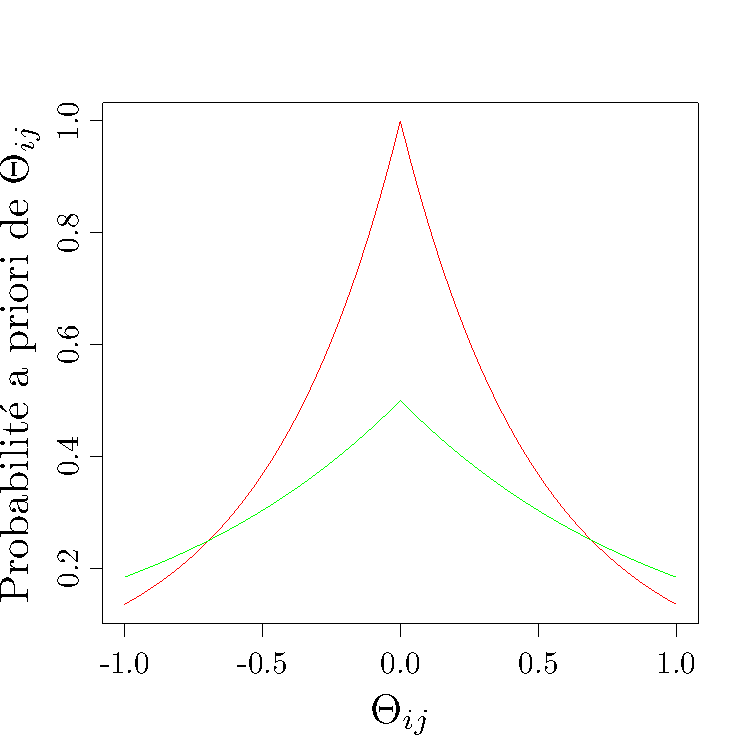
\includegraphics[width=.45\textwidth]{figures/laplacian_prior.pdf}
 %   \end{block}
 % 
 % \end{frame}

\begin{frame}
  \frametitle{How to come up with a latent clustering?}
  
  \begin{block}{Biological expertise}
    \begin{itemize}
    \item Build $\mathbf{Z}$ from prior biological information 
      \begin{itemize}
      \item transcription factors vs. regulatees,
      \item number of potential binding sites,
      \item KEGG pathways, \dots
      \end{itemize}
    \item Build the weight matrix from $\mathbf{Z}$.
    \end{itemize}
  \end{block}
  
  \vfill
  
  \begin{block}{Inference: Stochastic Bloc Model} 
    \begin{itemize}
    \item Spread the  nodes into $\mathcal{Q}$ classes;
    \item Connexion probabilities depend upon node classes:
      \begin{equation*}
        \mathbb{P} (i \leftrightarrow j|i \in \mathsf{ class}\ q, j \in
        \mathsf{ class }\ \ell) = \pi_{q \ell}.
      \end{equation*}
    \item Build $P_{\mathbf{Z}} \propto 1-\pi_{q\ell}$.
    \end{itemize}
   \end{block}
\end{frame}

\begin{frame}
  \frametitle{Illustration on breast Cancer}
  \framesubtitle{Prediction   of    the   outcome    of   preoperative
    chemotherapy}
  \begin{overlayarea}{\textwidth}{\textheight}
    \begin{columns}[c]
      \begin{column}{.35\textwidth}
        
        \begin{thebibliography}{99}
          \begin{footnotesize}
          \bibitem{hess}  Hess \textit{et  al.}   \newblock Journal.  of
            Clinical Oncology, 2006.
          \end{footnotesize}
        \end{thebibliography}
        
        \begin{block}{Data set}
          \small 133 patients classified as
          \begin{enumerate}
          \item \small pathologic complete response,
          \item \small residual disease,
          \end{enumerate}
          according to a signature of 26 genes (small network).
        \end{block}
      \end{column}
      
      \begin{column}{.65\textwidth}
        \begin{figure}
          \centering
          \includegraphics<1>[width=.9\textwidth]{hess_noclust}
          \includegraphics<2>[width=.9\textwidth]{breast_thirtyedges}
          \small\caption{Pooling the data, \only<1>{Neighborhood Selection}\only<2>{SIMoNE with clustering}}
        \end{figure}
      \end{column}
    \end{columns}
  \end{overlayarea}
  
\end{frame}
